\documentclass{article}
% PKGS START
\usepackage[utf8x]{inputenc}
\usepackage[english,russian]{babel}
\usepackage{cmap}
\usepackage{commath}
\usepackage{amsmath}
\usepackage{amsfonts}
\usepackage{mathtools}
\usepackage{amssymb}
\usepackage{parskip}
\usepackage{titling}
\usepackage{color}
\usepackage{hyperref}
\usepackage{cancel}
\usepackage{enumerate}
\usepackage{multicol}
\usepackage{graphicx}
\usepackage[a4paper, left=2.5cm, right=1.5cm, top=2.5cm, bottom=2.5cm]{geometry}
% PKGS END
% INIT START
\graphicspath{ {./images/} }
\setlength{\droptitle}{-3cm}
\hypersetup{
    colorlinks=true, %set true if you want colored links
    linktoc=all,     %set to all if you want both sections and subsections linked
    linkcolor=blue,  %choose some color if you want links to stand out
}

\pagenumbering{arabic}
% INIT END
\begin{document}
    % \begin{figure}[h!]
    % \centering
    % 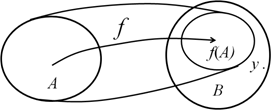
\includegraphics{2}
    % \caption{\label{fig:fig2}Разность и симметрическая разность множеств.}
    % \end{figure}
    \addtocontents{toc}{\protect\contentsline{section}{\protect\numberline{}Первый семестр}{}{}}
    \section{Пределы функций}
    \subsection{Теорема Вейерштрасса о предельной точке}

    \(\mathbb{E}\) --- числовое множество.

    \textbf{Определение.} Число \(a\) называется предельной точкой числового множества \(\mathbb{E}\), если \(\forall \varepsilon > 0\) в \\
    \(\varepsilon\)-окрестности точки \(a(U_\varepsilon(a))\ \exists\) хотя бы одна точка \(x\) из \(\mathbb{E};\ x \neq a\)

    \textbf{Определение.} Число \(a\) называется предельной точкой числового множества \(\mathbb{E}\),
    если в \(\forall U_\varepsilon(a)\) содержится \(\infty\) число элементов из \(\mathbb{E}\).

    \textbf{Теорема.} Если \(a\) --- предельная точка ч.м. \(\mathbb{E}\), то в \(\mathbb{E}\ \exists\ \{x_n\}:\ x_n \neq x_m, x_n \neq a \forall n:\ x_n \xrightarrow[n \rightarrow \infty]{} a\)

    \(\uparrow\) по определению 1

    \begin{enumerate}
        \item \(\varepsilon_{1} > 0 \xRightarrow[]{\textrm{Опр. 1}}\) в \(U_{\varepsilon_{1}}(a)\ \exists\ x_1:\ \begin{cases}x_1 \in \mathbb{E}\\ x_1 \neq a \end{cases}\) и \(\abs{x_1 - a} < \varepsilon_1\)
        \item \(\varepsilon_{2} \leq \frac{\abs{x_1 - a}}{2} \xRightarrow[]{\textrm{Опр. 1}}\) в \(U_{\varepsilon_{2}}(a)\ \exists\ x_2:\ \begin{cases}x_2 \in \mathbb{E}\\ x_2 \neq a \end{cases}\) и \(\abs{x_2 - a} < \varepsilon_2\)
        \item \(\varepsilon_3 \leq \frac{\abs{x_2-a}}{2} \xRightarrow[]{\textrm{Опр. 1}}\) в \(U_{\varepsilon_3}(a)\ \exists\ x_3:\ \begin{cases}x_3 \in \mathbb{E}\\ x_3 \neq a \end{cases}\) и \(\abs{x_3-a} < \varepsilon_3\)
        \item[$\vdots\;\;$]
        \item[$n$.] \(\varepsilon_{n} (> 0) \leq \frac{\abs{x_{n-1}}}{2} \xRightarrow[]{\textrm{Опр. 1}}\ \exists\ x_n: \begin{cases}x_n \in \mathbb{E}\\ x_n \neq a \end{cases}\) и \(\abs{x_n - a} < \varepsilon_{n}\)
        \item[$\vdots\;\;$]
    \end{enumerate}

    \(\Rightarrow \{x_n\}\)

    Осталось \(\{x_n\} \xrightarrow[]{\textrm{?}} a\)

    \(\forall\ \varepsilon > 0\ \exists\ N: \forall n > N: \abs{x_n - a} < \varepsilon\)

    \(\abs{x_n - a} < \varepsilon_n \leq \frac{\abs{x_{n-1}-a}}{2} < \frac{\varepsilon_{n-1}}{2} \leq \frac{\abs{x_{n-2}-a}}{2^2} < \frac{\varepsilon_{n-2}}{2^2} < ... < \frac{\varepsilon_{1}}{2^{n-1}} < \frac{\varepsilon_1}{n} < \varepsilon\)

    \(n > \frac{\varepsilon_1}{\varepsilon};\ N=[\frac{\varepsilon_1}{\varepsilon}] + 1\)

    \textbf{Замечание.} Верно и утверждение обратное к утверждению теоремы.

    \textbf{Определение 3} \(a\) --- предельная точка числового множества \(\mathbb{E} \Leftrightarrow\) когда в \(\mathbb{E}\ \exists\) последовательность различных \(x_n: x_n \neq a \forall n\) и \(x_n \xrightarrow[n \rightarrow \infty]{}\).

    Опр. 1 \(\Leftrightarrow\) Опр. 2 \(\Leftrightarrow\) Опр. 3

    \(a \in \mathbb{E}\) или \(a \not\in \mathbb{E}\)

    \begin{enumerate}
        \item \(\mathbb{E} = \{x=\frac{1}{n};\ n \in N\}\)

        \(a = 0\) --- предельная точка \(\mathbb{E}, a \not \in \mathbb{E}\)

        \item \(\mathbb{Q};\ \forall_q\) --- предельная точка

        \item \(\mathbb{N}\) нет предельных точек

        \item M --- конечное. Нет предельных точек
    \end{enumerate}

    \subsubsection{Теорема Вейерштрасса о предельной точке}
    Если бесконечное числовое множество \(\mathbb{E}\) ограничено, то для него существует хотя бы одна предельная точка.

    \(\uparrow\) Т.к. \(\mathbb{E}\) ограничено, \(\exists\ [m; M]:\ \mathbb{E} \subset  [m; M]\)

    \begin{enumerate}
        \item Делим \([m; M]:\ \begin{cases}[m; \frac{m+M}{2}]\\ [\frac{m+M}{2}; M]\end{cases}\)
        и выбираем ту часть, в которой содержится \(\infty\) число эл-тов из \(\mathbb{E}\), в ней берём какой-то \(x\)
        \item снова делим на 2 и в одной из частей берем \(x_2 \neq x_1\)
    \end{enumerate}
    и т.д. \(\Rightarrow \{x_n\} \in \mathbb{E}\)

    по теореме Больцано-Вейерштрасса(или вложенных промежутков) \(x_n\) -- сх-ся к \(a\).

    Это \(a\) --- предельная точка \(E\), по Опр.3.
    \(\downarrow\)

    \subsection{Предел функции в точке}

    \(y=f(x):\ X \rightarrow Y, a\) --- предельная точка \(X:\ \lim_{x \rightarrow a}{f(x)} = A\)

    \textbf{Определение.} Будем говорить, что существует предел функции f(x) при \(x \rightarrow a\) \( (lim_{x\rightarrow a}) = A) \), если

    \begin{enumerate}
        \item функция \(f(x)\) определена в некоторой окрестности точки \(x=a\); за исключением, возможно, самой \(x=a\)
        \item \(\forall \varepsilon > 0 \exists\ \delta(\varepsilon): \forall x: 0 < \abs{x - a} < \delta\) выполняется \(\abs{f(x) - A} < \varepsilon\).
    \end{enumerate}
    \(a - \delta < x < a + \delta\ x \neq a\).

    \(A - \varepsilon < f(x) < A + \varepsilon\)

    \textbf{Отрицание} \(\exists \varepsilon > 0: \forall \delta(\varepsilon) \exists x: 0 < \abs{x - a} < \delta\) и \(\abs{f(x) - A} \geq \varepsilon\)

    \textbf{Определение.} Будем говорить, что существует предел функции f(x) при \(x \rightarrow a\) \( (lim_{x\rightarrow a}) = A);\ f(x) \xrightarrow[x \rightarrow a]{} A\); если

    \begin{enumerate}
      \item \(f(x)\) определено в \(U_\delta(a)\)
      \item \(\forall x_n \rightarrow a \Rightarrow y_n = f(x_n)\rightarrow A\)
    \end{enumerate}
    (Определение по Гейне)

    Доказательство экв Опр. 1 \(\Leftrightarrow\) Опр. 2:
    \(\uparrow\)
    \begin{enumerate}
      \item \(\Rightarrow\) из Опр. 1 \(\Rightarrow\) Опр. 2\\
      надо, что если \(\forall x_n \rightarrow a \Rightarrow y_n = f(x_n) \rightarrow A\)

      ? (\(\forall \varepsilon > 0 \exists\ N: \forall n > N \abs{f(x) - A} < \varepsilon\))

      \(\forall \varepsilon > 0 \xRightarrow[]{\textrm{Опр.1}}\ \exists\ \delta(\varepsilon):\) по \(\delta(\varepsilon)\) т.к. \(x_n \rightarrow a\).\\
      \(\exists\ N:\ \forall n > N\ \abs{x_n-a}<\delta \xRightarrow[]{\textrm{Опр.1}} \abs{f(x_n)-A}<\varepsilon\)

      \item \(\Leftarrow\) дано \(\forall x_n \rightarrow a\ f(x) \rightarrow A\).\\ От противного. Пусть Опр.1 не выполняется, т.е.
      \(\exists\ \varepsilon > 0:\ \forall \delta\ \exists\ x:\ 0 < \abs{x-a}<\delta\), но \(\abs{f(x)-A}\geq \varepsilon\).

      Рассмотрим \(\delta_k = \frac{1}{k}, k \in \mathbb{N},\) тогда \(\exists\ x_k:\ 0<\abs{x_k-a}<\delta=\frac{1}{k}\)
      \begin{equation*}
        a-\frac{1}{k}<x_k<a+\frac{1}{k}(*)
      \end{equation*}

      \(x_k\) --- сх-ся, \(f(x_k)\) (*) --- расх-ся (против Опр. 2)
      \(\downarrow\)
    \end{enumerate}
\end{document}
